Different sources provide different data to the company.
Some information are stored in specific databases, while other data first need to be processed by specific tools before being stored.
In several cases, databases store both the raw data and the results of the computations performed by specific tools.

\begin{figure}
    \centering
    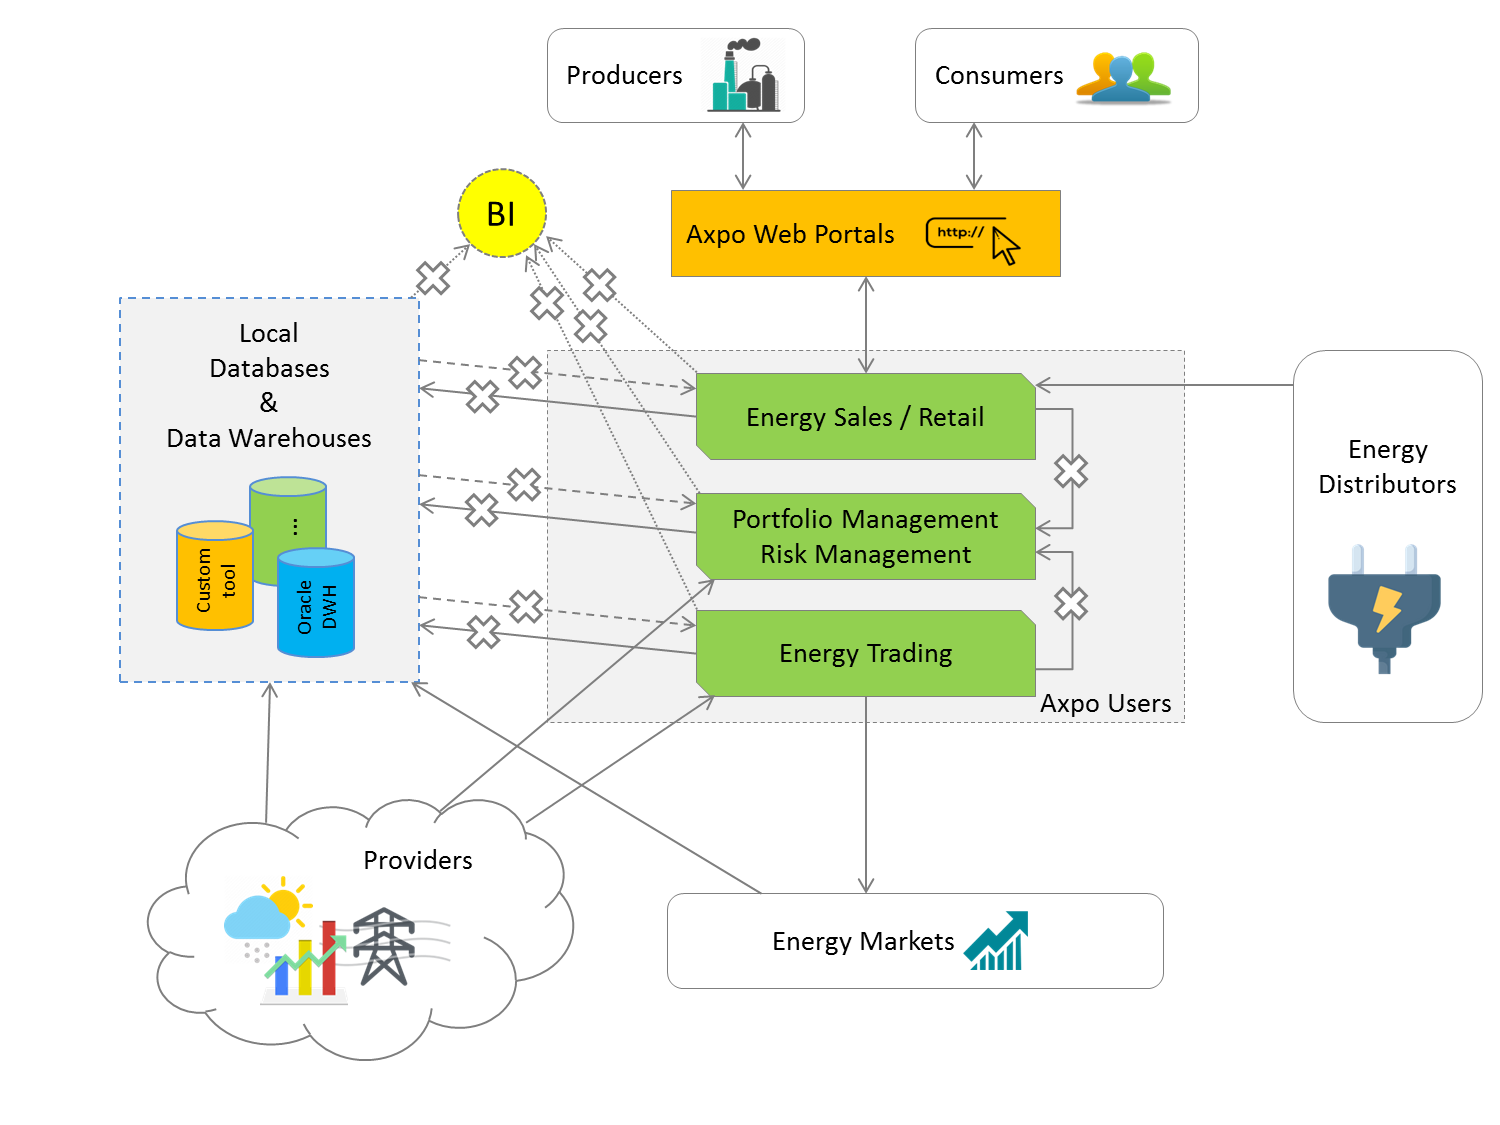
\includegraphics[width=\textwidth]{res/architecture/arch_start.png}
    \caption{
        Current data communication structure among Axpo departments and data sources.\\
        X's represent integration software.
    }
    \label{fig:architecture:start}
\end{figure}

Figure \ref{fig:architecture:start} shows an overview of data communication among Axpo departments and the different external data sources.

As we can see, each department communicates with multiple local databases, as well as with other departments.
All these communications are mediated by several pieces of integration software (represented by X's in the figure).

The data is stored in a few databases, which are used by several departments and contain several kinds of information.
All these databases are on-premise.
This brings several advantages, such as a great degree of availability and ease of management, but has also some problems, which have become more and more relevant in the last years.
These problems are related to database performances and data quality as well as to the management of the processes used to communicate with the databases.

\subsection{Integration Software}
    One of the most apparent issues is the high quantity of integration software used by the company.
    
    Each department needs data in a specific format.
    Often the information are stored differently.
    During retrieval, custom programs are used to manipulate data in advanced ways, for example by merging results from a query with information from a different source or by performing cleaning operations too complex to be expressed in SQL.

    \paragraph{Management}
        A few years ago, the quantity of integration software was low and easy to manage.
        However, as the company grew, more programs have been added and the situation has become harder and harder to manage.
        The company does not have some kind of documentation or schema which can be consulted to understand which programs are used and what they do.
        
        Sometimes subscriptions are paid for tools which are no longer needed, since a new tool could do the same things.
        However, the high complexity of the system and the lack of documentation can make this problem difficult to notice.
        
    \paragraph{Performance}
        Having a high number of tools means that data must go through several steps.
        Sometimes multiple tools are required for the needs of specific users.
        
        This has an obvious impact on performance, since a large number of computations is performed on the data.
        
    \paragraph{Bug tracing}
        Given the high number of tools, if an issue is found with some data, it is extremely difficult to trace its cause, since it could reside in any of the tools used in the process.
        
        As a consequence, debugging may become a very complex and time-consuming activity.

\subsection{Database Performance}
    The databases has been slowing down over the last years, given the constantly increasing amount of data.
    Some tables contain hundreds of millions of records, which sometime make even performing simple queries a long operation.
    
    In some cases, performing a simple query (for example with two equality checks on the \code{WHERE} clause) can take up to a few minutes.
    
    These long execution times have become problematic in some critical processes, which have to be completed daily before a specific time.
    
\subsection{Data Quality}
    An additional problem was related to data quality.
    
    There were no data quality assurance processes in-place, which means there was no way to validate the quality of new data.
    
    This led to data cleaning operations executed directly into the queries, which severely impacted performances negatively.
    
    For example, some users needed to extract data related to the energy production of some UPs\footnote{
        \textit{Unità di produzione} (Production Unit).
        An UP is a plant which produces electric energy.
    }.
    The information are stored on a single table, but presented many problems related to data quality.
    
    The main issues are:
    \paragraph{Inconsistent plant names}
        There is no quality assurance control when receiving plant names from providers.
        These names are most likely manually input by clients, since we noticed they sometimes contain typos.
        
        For example a specific UP, called \textit{UP\_ParcoEolico\_1} was one time named \textit{UP\_ParcoElico\_1}.
        
        Table \ref{tab:sbil:up_names} shows some naming inconsistencies.
        
        \begin{table}
            \centering
            \begin{tabular}{|l l|}
                \toprule
                Actual name         & Correct name      \\
                \midrule
                IM\_020****         & IM\_20****        \\
                IM\_0S1****         & IM\_S1****        \\
                \midrule
                IM\_036****         & PVI\_036****\_001 \\
                IM\_036****\_01     & PVI\_036****\_001 \\
                \midrule
                UP\_PARCOELICO\_1    & UP\_PARCOEOLICO\_1 \\
                UP\_PARCOEOLICO\_1   & UP\_PARCOEOLICO\_1 \\
                \bottomrule
            \end{tabular}
            \caption{Some UP naming inconsistencies.}
            \label{tab:sbil:up_names}
        \end{table}

    \paragraph{Different date conventions}
        Each provider handles DST\footnote{
            \textit{Daylight Saving Time}.
             Several countries advance clocks during summer months so that evening daylight lasts longer, while sacrificing normal sunrise times.
        } changes in a different way\footnote{
            During DST changes we can either have 23 or 25 hours in a single day.
            In the first case, some provider name the hours from 0 to 23, while others may keep the standard 24 hour format but skip the hour 2.
            In the second case, some providers use a 25 hours notation, while others call the hours when the change occurs 3A and 3B.
            There are also several providers which don't use any of the above notations but have their own specific format.
        }.
        The main issues are that there are no normalization actions in-place and that data from different providers are stored in the same table.
        
        This causes a problem when extracting data from the table, since each provider needs \textit{ad hoc} logic in the query, which not only makes it harder to read, but also negatively impacts performance.
        
        As an example, let us consider a query needing to extract information from a table containing data from two weather forecast providers, say \textit{Provider A} and \textit{Provider B}\footnote{
            The actual names of the providers are trade secrets and, as a consequence, cannot appear in this document.
        }.
        However, the two providers handle DST in different ways.
        Upon further analysis, we discovered that even a single provider doesn't have a consistent approach across all years.
        
        In detail, we have:
            \begin{itemize}
                \item Lack of consistency across providers
                \item Lack of consistency across different years of the same provider
            \end{itemize}

        For example, the day when DST ends we are supposed to have 25 hours, since the hour between 2 and 3 a.m. is repeated twice.
        
        The data provided by \textit{Provider A} are ranged 1 to 25, which is what mathematical models expect, while \textit{Provider B} only provides 24 hours and discards the 25th.
        In this case it is necessary to remap all the hours after 2 a.m., which is when the DST change occurred.
        
        The behavior of \textit{Provider B} isn't however consistent across all years, since we noticed that the data prior to 2017 have 25 hours.
        As such it is important to take into account the year when deciding whether to remap the hours or not.
        
    \paragraph{Data scattering}
        These tables are populated with data from several different sources.
        
        For example, a consistent number of information are extracted from a custom tool which acts as a database, but has many more functionalities.
        However, the data contained in this custom tool comes from a different one, \textit{Trimp}, which is a metering tool\footnote{
            A metering tool regularly receives values from energy meters and performs some basic operations on them depending on the meter type.
            For example old meters send a cumulative count of how much energy has been consumed since the meter was installed, while newer models only send the amount consumed since the last reading.
        } developed by a third-party organization.
        
        This high interaction between tools adds an additional layer of complexity to the system, impacting negatively both performance and understanding.
        
    \paragraph{Long execution times}
        Some queries contain several \code{CASE ... WHEN ...} instructions, sometimes even with multiple nested \code{SUBSTRING} and \code{CHARINDEX} operations.
        These data cleaning operations severely impact performances, since the database has to perform long operations for each record.
        
        \begin{figure}
            \centering
            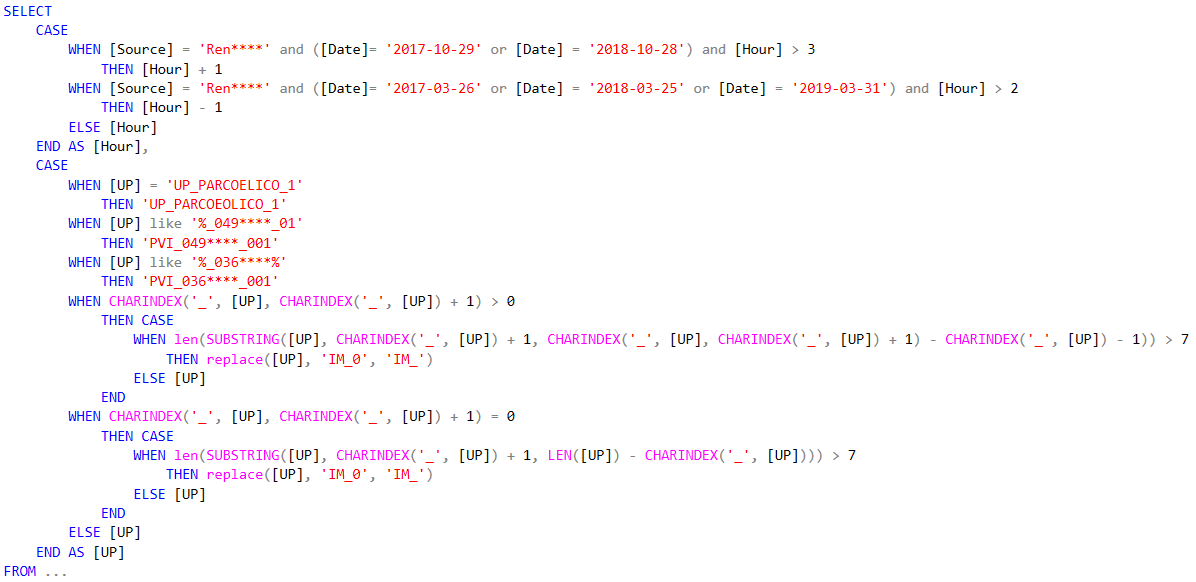
\includegraphics[width=\textwidth]{res/bigdata_query_casewhen.png}
            \caption{Data cleaning operations performed in-query.}
            \label{fig:query_cleanup_casewhen}
        \end{figure}
        
        Figure \ref{fig:query_cleanup_casewhen} shows an example of cleaning operations performed in the query.
        
        On the other hand, if there had been some data quality guarantee, these queries could have been greatly simplified and their performance would have improved greatly.
        
        For example, the query shown in Figure \ref{fig:query_cleanup_casewhen} would have simply become \code{SELECT [Hour], [UP] FROM ...}.
        In this case, this query could also benefit from indexing, while in the current state this situation is impossible, since indexes do not work when data are manipulated (for example by a \code{SUBSTRING} operation).
